\section{Introduction}
\label{sec:intro}

\begin{figure}[h]
\vskip -.7cm
    \centering
    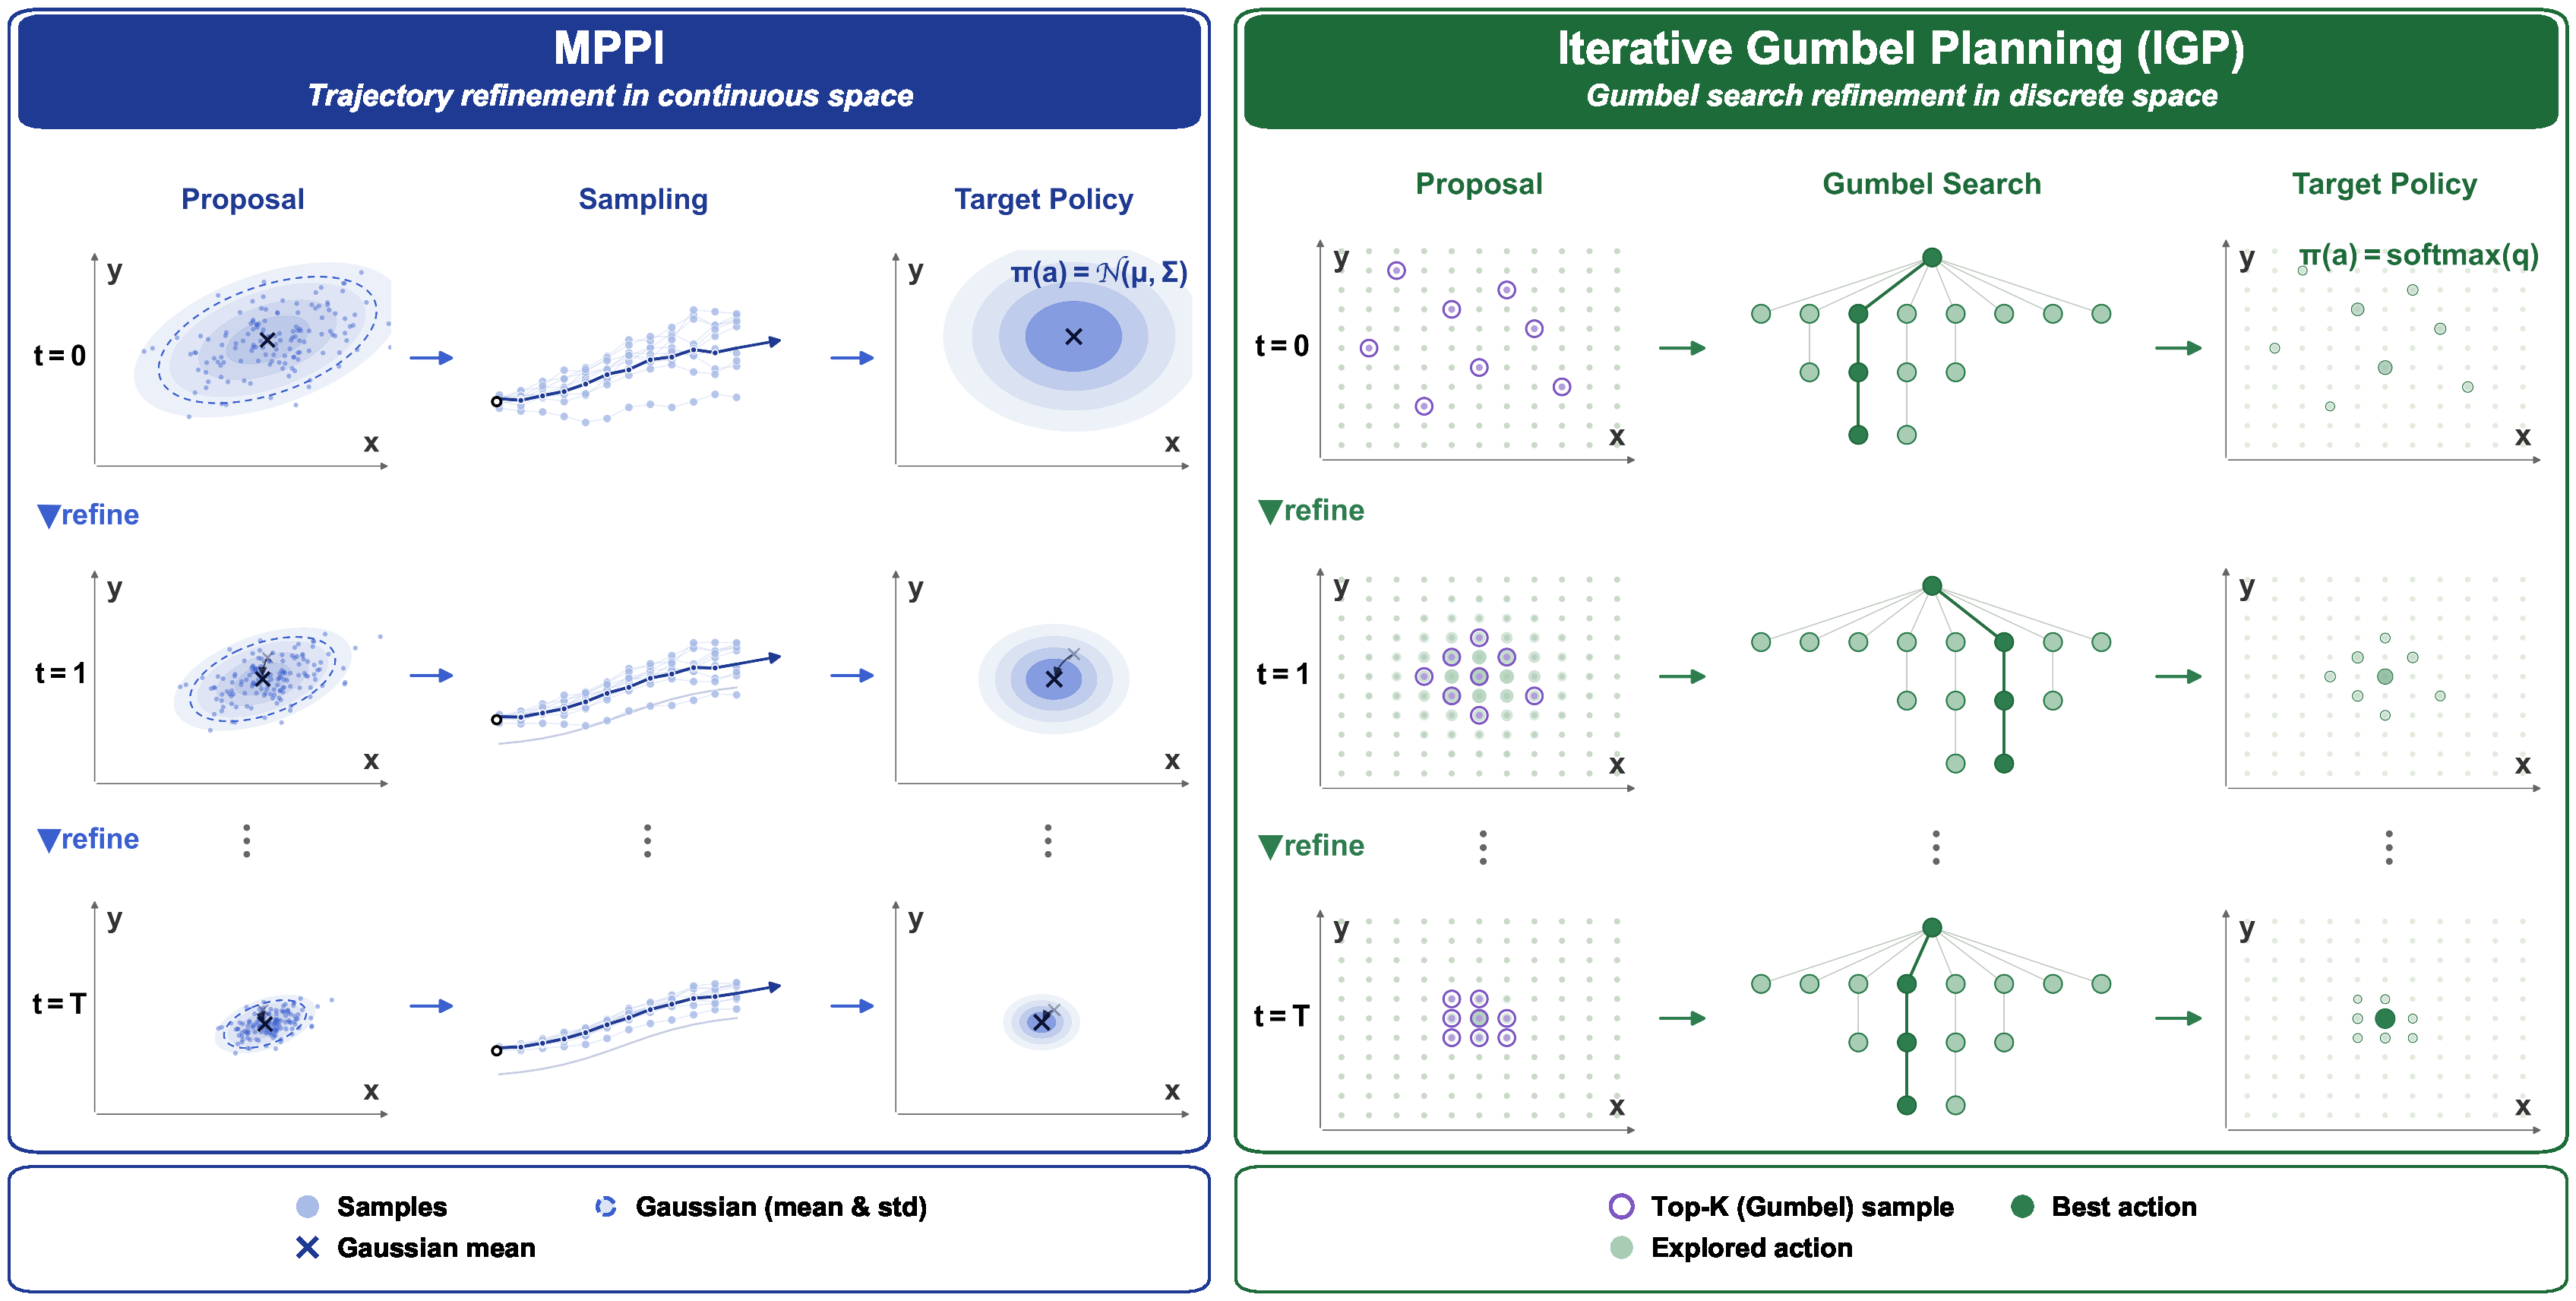
\includegraphics[width=0.95\linewidth]{figs/method.pdf}
    \caption{\textbf{Comparison of MPPI and Iterative Gumbel Planning (IGP).} While standard MPPI refines trajectories over an unbounded continuous action space, IGP natively operates in a factorized discrete policy space. By utilizing per-dimension Gumbel Top-$K$ sampling, IGP executes multi-round iterative search to systematically refine a categorical root policy at each state.}
    \vskip -.3cm
    \label{fig:method}
\end{figure}

\begin{wrapfigure}{r}{0.5\textwidth}
    \centering
    \vspace{-10pt}
    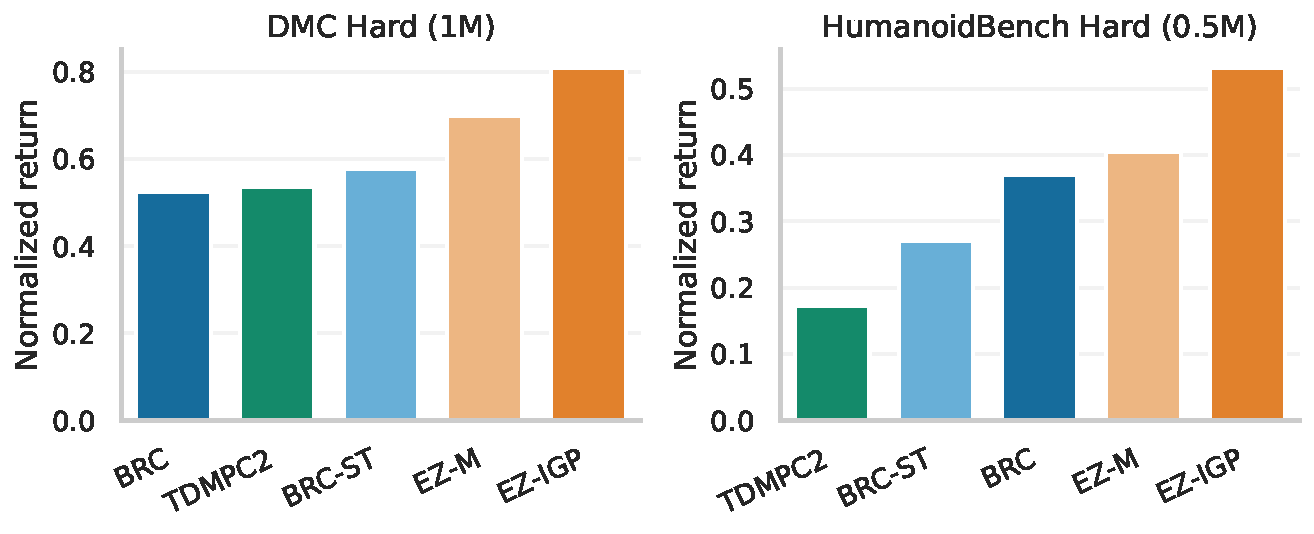
\includegraphics[width=0.49\textwidth]{figs/fig1_overall_igp_bar.pdf}
    \caption{\textbf{Factorized policies achieve SOTA performance.} Across high-dimensional continuous-control benchmarks, our iteratively refined policy consistently attains strong returns. \textcolor{blue}{These results support factorized discrete representations with iterative search as a practical alternative to Gaussian proposals on the evaluated tasks.}}
    \label{fig:overall_bar}
    \vspace{-10pt}
\end{wrapfigure}

Continuous control is a key challenge for reinforcement learning, with applications across robotics, control, and beyond. The dominant difficulty lies in credit assignment over long horizons in high-dimensional action spaces. Search-based planning offers a principled response: by combining a learned model with value-guided lookahead, it propagates value estimates over multiple steps and selects actions through explicit comparison rather than single-step bootstrapping. This paradigm has driven major progress on discrete-action benchmarks, with the AlphaGo and MuZero families~\citep{silver2017mastering, schrittwieser2020mastering, hubert2021learning, danihelka2022policy, ye2021mastering} setting the state of the art. Extending it to continuous control is therefore natural, and recent work has begun to explore this direction~\citep{hubert2021learning, wang2024efficientzero}. Yet the continuous setting has not seen comparable dominance, and we argue that the reason lies in a structural mismatch between search and the policy class.

Search is fundamentally a discrete improvement operator: at each state, it evaluates a finite set of candidate actions and returns a categorical distribution over them. In contrast, existing search-based continuous-control methods inherit Gaussian policies from policy-gradient RL~\citep{lillicrap2019continuouscontroldeepreinforcement, haarnoja2018soft} and distill the search output into them via maximum likelihood. Since the selected action is sampled from the Gaussian and rarely coincides with its mean, maximum likelihood not only shifts the mean toward the target but can also encourage larger variance to cover the sampled candidate. We show that winner-action distillation produces a stepwise variance-expanding gradient tendency when the selected action is sufficiently far from the current mean. \textcolor{blue}{Figure~\ref{fig:var_comp}(a) further demonstrates its sustained training-time consequence: the Gaussian standard deviation rises early and remains elevated throughout the observed training horizon.}

To remove this projection error, the policy should be structurally aligned with the discrete search output. A natural solution is to discretize the continuous action space. Although discretization introduces its own approximation gap, we show that this gap is bounded and controllable by the grid resolution, replacing the non-vanishing Gaussian projection error with an explicitly characterized discretization error. The key remaining challenge is the $V^{|A|}$ combinatorial explosion of joint discretization, which has prevented this idea from scaling to high-dimensional control domains.

To resolve this bottleneck, we propose \textbf{Iterative Gumbel Planning (IGP)}. IGP operates on a per-dimension factorized categorical policy, keeping the parameter count linear in $|A|$ while aligning the policy support with the search operator. \textcolor{blue}{Each dimension is sampled without replacement and equally ranked samples are aligned to form $K$ joint candidates. This is a scalable structured approximation, not exact without-replacement sampling from the exponentially large joint factorized distribution.} Crucially, IGP treats search not as a single-pass procedure, but as an MPPI-style multi-round refinement process that repeatedly improves the root policy at the same state.

We implement IGP on EfficientZero-Multitask (EZ-M)~\citep{liu2026scaling} and evaluate it on DMControl~\citep{tassa2018deepmind} and HumanoidBench~\citep{sferrazza2024humanoidbench}, covering high-dimensional locomotion and whole-body humanoid control. IGP achieves state-of-the-art performance, improves sample efficiency over strong model-based baselines, and produces action sequences with lower temporal variance at evaluation, which is relevant to real-world robotic deployment. Qualitative rollouts comparing Gaussian and IGP are available at \href{https://mellifluous-marzipan-a1cb45.netlify.app/}{this anonymous website}. \textbf{Our contributions are}: (1) We characterize the variance-expanding gradient tendency induced by winner-action Gaussian distillation and contrast its projection error with the bounded, controllable error of discretization; (2) We propose Iterative Gumbel Planning (IGP), which performs MPPI-style multi-round refinement over a factorized categorical policy via Gumbel Top-$K$ sampling, bypassing Gaussian projection; (3) IGP achieves state-of-the-art sample efficiency on DMControl and HumanoidBench, yielding significantly lower temporal action variance and smoother control behaviors at evaluation.
